\documentclass[11pt,a4paper]{ctexart}

\usepackage[margin=2.2cm]{geometry}
\usepackage{booktabs}
\usepackage{float}
\usepackage{graphicx}
\usepackage[unicode,hidelinks,bookmarksopen,bookmarksdepth=2]{hyperref}

\begin{document}

\setcounter{secnumdepth}{2}

\section{GenRec-Only Tables}

本文件由 \texttt{build\_genrec\_only\_tables.py} 自动生成。本轮重排按 \texttt{RQ1--RQ4} 组织，只保留当前 index 下已测到的 GenRec 系列结果，并把 full curves / first-epoch tables 统一放到 appendix。

\tableofcontents
\newpage

\section{RQ1: Overall Performance}

这一节沿用当前默认口径：每个变体都在其全部已同步 checkpoint 中按 \texttt{NDCG@10} 选出唯一 best checkpoint。 Games 仍保留当前已有的主线五列；Instruments 与 Arts 额外纳入 \texttt{ce0.001 / ce0.01}，从而把 overall frontier 一次放全。

\subsection{Instruments}

\begin{table}[H]
\centering
\scriptsize
\setlength{\tabcolsep}{4pt}
\renewcommand{\arraystretch}{1.08}
\resizebox{\textwidth}{!}{%
\begin{tabular}{lccccccc}
\toprule
Metric & GenRec(sft) & GenRec(rule) & GenRec(ranking) & GenRec(fixed) & GenRec(fixed + ce0.001) & GenRec(fixed + ce0.005) & GenRec(fixed + ce0.01) \\
\midrule
HR@1 & 0.0588 & \underline{0.0788} & \textbf{0.0808} & 0.0722 & 0.0747 & 0.0764 & 0.0761 \\
HR@5 & 0.0932 & \textbf{0.1027} & 0.1002 & 0.1014 & 0.0993 & 0.1009 & \underline{0.1016} \\
HR@10 & 0.1094 & 0.1179 & 0.1145 & \underline{0.1189} & 0.1168 & 0.1180 & \textbf{0.1204} \\
HR@20 & 0.1344 & 0.1373 & 0.1337 & 0.1447 & \underline{0.1449} & 0.1435 & \textbf{0.1456} \\
HR@50 & 0.1844 & 0.1681 & 0.1696 & 0.1941 & \underline{0.1951} & \textbf{0.1985} & 0.1943 \\
NDCG@5 & 0.0771 & \textbf{0.0911} & \underline{0.0906} & 0.0875 & 0.0875 & 0.0890 & 0.0893 \\
NDCG@10 & 0.0823 & \textbf{0.0960} & 0.0952 & 0.0931 & 0.0931 & 0.0945 & \underline{0.0953} \\
NDCG@20 & 0.0886 & \underline{0.1009} & 0.1000 & 0.0995 & 0.1002 & \underline{0.1009} & \textbf{0.1016} \\
NDCG@50 & 0.0985 & 0.1070 & 0.1071 & 0.1094 & 0.1102 & \textbf{0.1118} & \underline{0.1113} \\
\midrule
Selected ckpt & \texttt{checkpoint-495} & \texttt{checkpoint-2997} & \texttt{checkpoint-1665} & \texttt{checkpoint-2997} & \texttt{checkpoint-2664} & \texttt{checkpoint-1665} & \texttt{checkpoint-2997} \\
\bottomrule
\end{tabular}%
}
\caption{Instruments 上仅保留 GenRec 系列方法的结果。}
\label{tab:genrec-only-instruments}
\end{table}

\subsection{Games}

\begin{table}[H]
\centering
\scriptsize
\setlength{\tabcolsep}{4pt}
\renewcommand{\arraystretch}{1.08}
\resizebox{\textwidth}{!}{%
\begin{tabular}{lccccc}
\toprule
Metric & GenRec(sft) & GenRec(rule) & GenRec(ranking) & GenRec(fixed) & GenRec(fixed + ce0.005) \\
\midrule
HR@1 & 0.0168 & \underline{0.0206} & 0.0203 & \textbf{0.0210} & \textbf{0.0210} \\
HR@5 & 0.0503 & 0.0544 & 0.0541 & \underline{0.0555} & \textbf{0.0558} \\
HR@10 & 0.0804 & \underline{0.0825} & 0.0802 & \textbf{0.0857} & \textbf{0.0857} \\
HR@20 & 0.1215 & 0.1186 & 0.1167 & \underline{0.1273} & \textbf{0.1278} \\
HR@50 & \underline{0.1998} & 0.1815 & 0.1804 & 0.1972 & \textbf{0.2012} \\
NDCG@5 & 0.0336 & 0.0377 & 0.0374 & \underline{0.0383} & \textbf{0.0385} \\
NDCG@10 & 0.0433 & \underline{0.0467} & 0.0458 & \textbf{0.0480} & \textbf{0.0480} \\
NDCG@20 & 0.0536 & 0.0558 & 0.0550 & \underline{0.0584} & \textbf{0.0586} \\
NDCG@50 & 0.0691 & 0.0683 & 0.0676 & \underline{0.0723} & \textbf{0.0732} \\
\midrule
Selected ckpt & \texttt{checkpoint-768} & \texttt{checkpoint-8752} & \texttt{checkpoint-3504} & \texttt{checkpoint-8752} & \texttt{checkpoint-3504} \\
\bottomrule
\end{tabular}%
}
\caption{Games 上当前已测到的 GenRec 系列结果。}
\label{tab:genrec-only-games}
\end{table}

\subsection{Arts}

\begin{table}[H]
\centering
\scriptsize
\setlength{\tabcolsep}{4pt}
\renewcommand{\arraystretch}{1.08}
\resizebox{\textwidth}{!}{%
\begin{tabular}{lccccccc}
\toprule
Metric & GenRec(sft) & GenRec(rule) & GenRec(ranking) & GenRec(fixed) & GenRec(fixed + ce0.001) & GenRec(fixed + ce0.005) & GenRec(fixed + ce0.01) \\
\midrule
HR@1 & 0.0643 & \textbf{0.0743} & 0.0728 & 0.0730 & 0.0710 & 0.0720 & \underline{0.0734} \\
HR@5 & 0.0949 & 0.1031 & 0.1018 & \underline{0.1041} & 0.1031 & \textbf{0.1048} & 0.1025 \\
HR@10 & 0.1164 & 0.1215 & 0.1189 & \underline{0.1248} & 0.1244 & \textbf{0.1257} & 0.1216 \\
HR@20 & 0.1433 & 0.1454 & 0.1412 & 0.1504 & \textbf{0.1537} & \underline{0.1518} & 0.1496 \\
HR@50 & 0.1941 & 0.1906 & 0.1839 & \underline{0.2007} & \textbf{0.2029} & 0.2006 & 0.1978 \\
NDCG@5 & 0.0801 & \textbf{0.0893} & 0.0876 & \underline{0.0890} & 0.0874 & 0.0889 & 0.0884 \\
NDCG@10 & 0.0870 & \underline{0.0952} & 0.0931 & \textbf{0.0956} & 0.0943 & \textbf{0.0956} & 0.0946 \\
NDCG@20 & 0.0938 & 0.1012 & 0.0987 & \textbf{0.1021} & \underline{0.1017} & \textbf{0.1021} & 0.1016 \\
NDCG@50 & 0.1038 & 0.1102 & 0.1071 & \textbf{0.1120} & 0.1114 & \underline{0.1118} & 0.1111 \\
\midrule
Selected ckpt & \texttt{checkpoint-522} & \texttt{checkpoint-2105} & \texttt{checkpoint-1684} & \texttt{checkpoint-3368} & \texttt{checkpoint-2105} & \texttt{checkpoint-2105} & \texttt{checkpoint-4206} \\
\bottomrule
\end{tabular}%
}
\caption{Arts 上当前已测到的 GenRec 系列结果。}
\label{tab:genrec-only-arts}
\end{table}

\section{RQ2: Deep Analysis for Prefix Hint}

这一节聚焦两个问题：其一，hint-conditioned training signal 是否真的有效；其二，prefix hint strategy 在 fixed / adaptive 与 task-aware / first-token 两个轴上如何比较。

\subsection{Hint-conditioned Training Signal}

先把问题压缩到最核心的四条线：\texttt{GenRec(sft)}、\texttt{Rule-only baseline}、\texttt{Adaptive hinting} 和 \texttt{Ours(3-task)}。

\begin{table}[H]
\centering
\scriptsize
\setlength{\tabcolsep}{4pt}
\renewcommand{\arraystretch}{1.08}
\begin{tabular}{lcccc}
\toprule
Metric & GenRec(sft) & Rule-only baseline & Adaptive hinting & Ours (3-task) \\
\midrule
HR@1 & 0.0588 & \textbf{0.0788} & \underline{0.0760} & 0.0722 \\
HR@5 & 0.0932 & \textbf{0.1027} & 0.0997 & \underline{0.1014} \\
HR@10 & 0.1094 & \underline{0.1179} & 0.1169 & \textbf{0.1189} \\
HR@20 & 0.1344 & 0.1373 & \underline{0.1394} & \textbf{0.1447} \\
HR@50 & 0.1844 & 0.1681 & \underline{0.1855} & \textbf{0.1941} \\
NDCG@5 & 0.0771 & \textbf{0.0911} & \underline{0.0880} & 0.0875 \\
NDCG@10 & 0.0823 & \textbf{0.0960} & \underline{0.0936} & 0.0931 \\
NDCG@20 & 0.0886 & \textbf{0.1009} & 0.0992 & \underline{0.0995} \\
NDCG@50 & 0.0985 & 0.1070 & \underline{0.1083} & \textbf{0.1094} \\
\midrule
Selected ckpt & \texttt{checkpoint-495} & \texttt{checkpoint-2997} & \texttt{checkpoint-2997} & \texttt{checkpoint-2997} \\
\bottomrule
\end{tabular}
\caption{Instruments 上 hint-conditioned training signal 的第一层证据。}
\label{tab:genrec-only-instruments-prefix-hint-signal}
\end{table}

\texttt{Rule-only baseline} 继续提供最高的无 hint top-10，但 \texttt{Adaptive hinting} 和 \texttt{Ours(3-task)} 都把 coverage 拉回到了 SFT 以上；这说明 prefix hint 的训练信号不是表面装饰，而是会真实改变 RL frontier 的形状。

\subsection{Hint Strategy Comparison}

这里直接比较四条你当前最关心的线：\texttt{Ours(fixed hint)}、\texttt{dynamic hint}、\texttt{fixed hint max1} 与 \texttt{dynamic hint max1}。这组对照把 fixed / dynamic 与 full-hint / max1 两个轴放进同一张表。

\begin{table}[H]
\centering
\scriptsize
\setlength{\tabcolsep}{4pt}
\renewcommand{\arraystretch}{1.08}
\begin{tabular}{lcccc}
\toprule
Metric & Ours (fixed hint) & Dynamic hint & Fixed hint max1 & Dynamic hint max1 \\
\midrule
HR@1 & 0.0722 & \underline{0.0760} & 0.0743 & \textbf{0.0761} \\
HR@5 & \underline{0.1014} & 0.0997 & \textbf{0.1017} & 0.0992 \\
HR@10 & \underline{0.1189} & 0.1169 & \textbf{0.1205} & 0.1158 \\
HR@20 & \underline{0.1447} & 0.1394 & \textbf{0.1456} & 0.1402 \\
HR@50 & \textbf{0.1941} & 0.1855 & \underline{0.1935} & 0.1905 \\
NDCG@5 & 0.0875 & 0.0880 & \textbf{0.0885} & \underline{0.0881} \\
NDCG@10 & 0.0931 & \underline{0.0936} & \textbf{0.0945} & 0.0934 \\
NDCG@20 & \underline{0.0995} & 0.0992 & \textbf{0.1008} & \underline{0.0995} \\
NDCG@50 & 0.1094 & 0.1083 & \textbf{0.1103} & \underline{0.1095} \\
\midrule
Selected ckpt & \texttt{checkpoint-2997} & \texttt{checkpoint-2997} & \texttt{checkpoint-2652} & \texttt{checkpoint-1332} \\
\bottomrule
\end{tabular}
\caption{Instruments 上 \texttt{Ours(fixed hint)}、\texttt{dynamic hint}、\texttt{fixed hint max1} 与 \texttt{dynamic hint max1} 的对比。}
\label{tab:genrec-only-instruments-hint-comparison}
\end{table}

\begin{figure}[p]
\centering
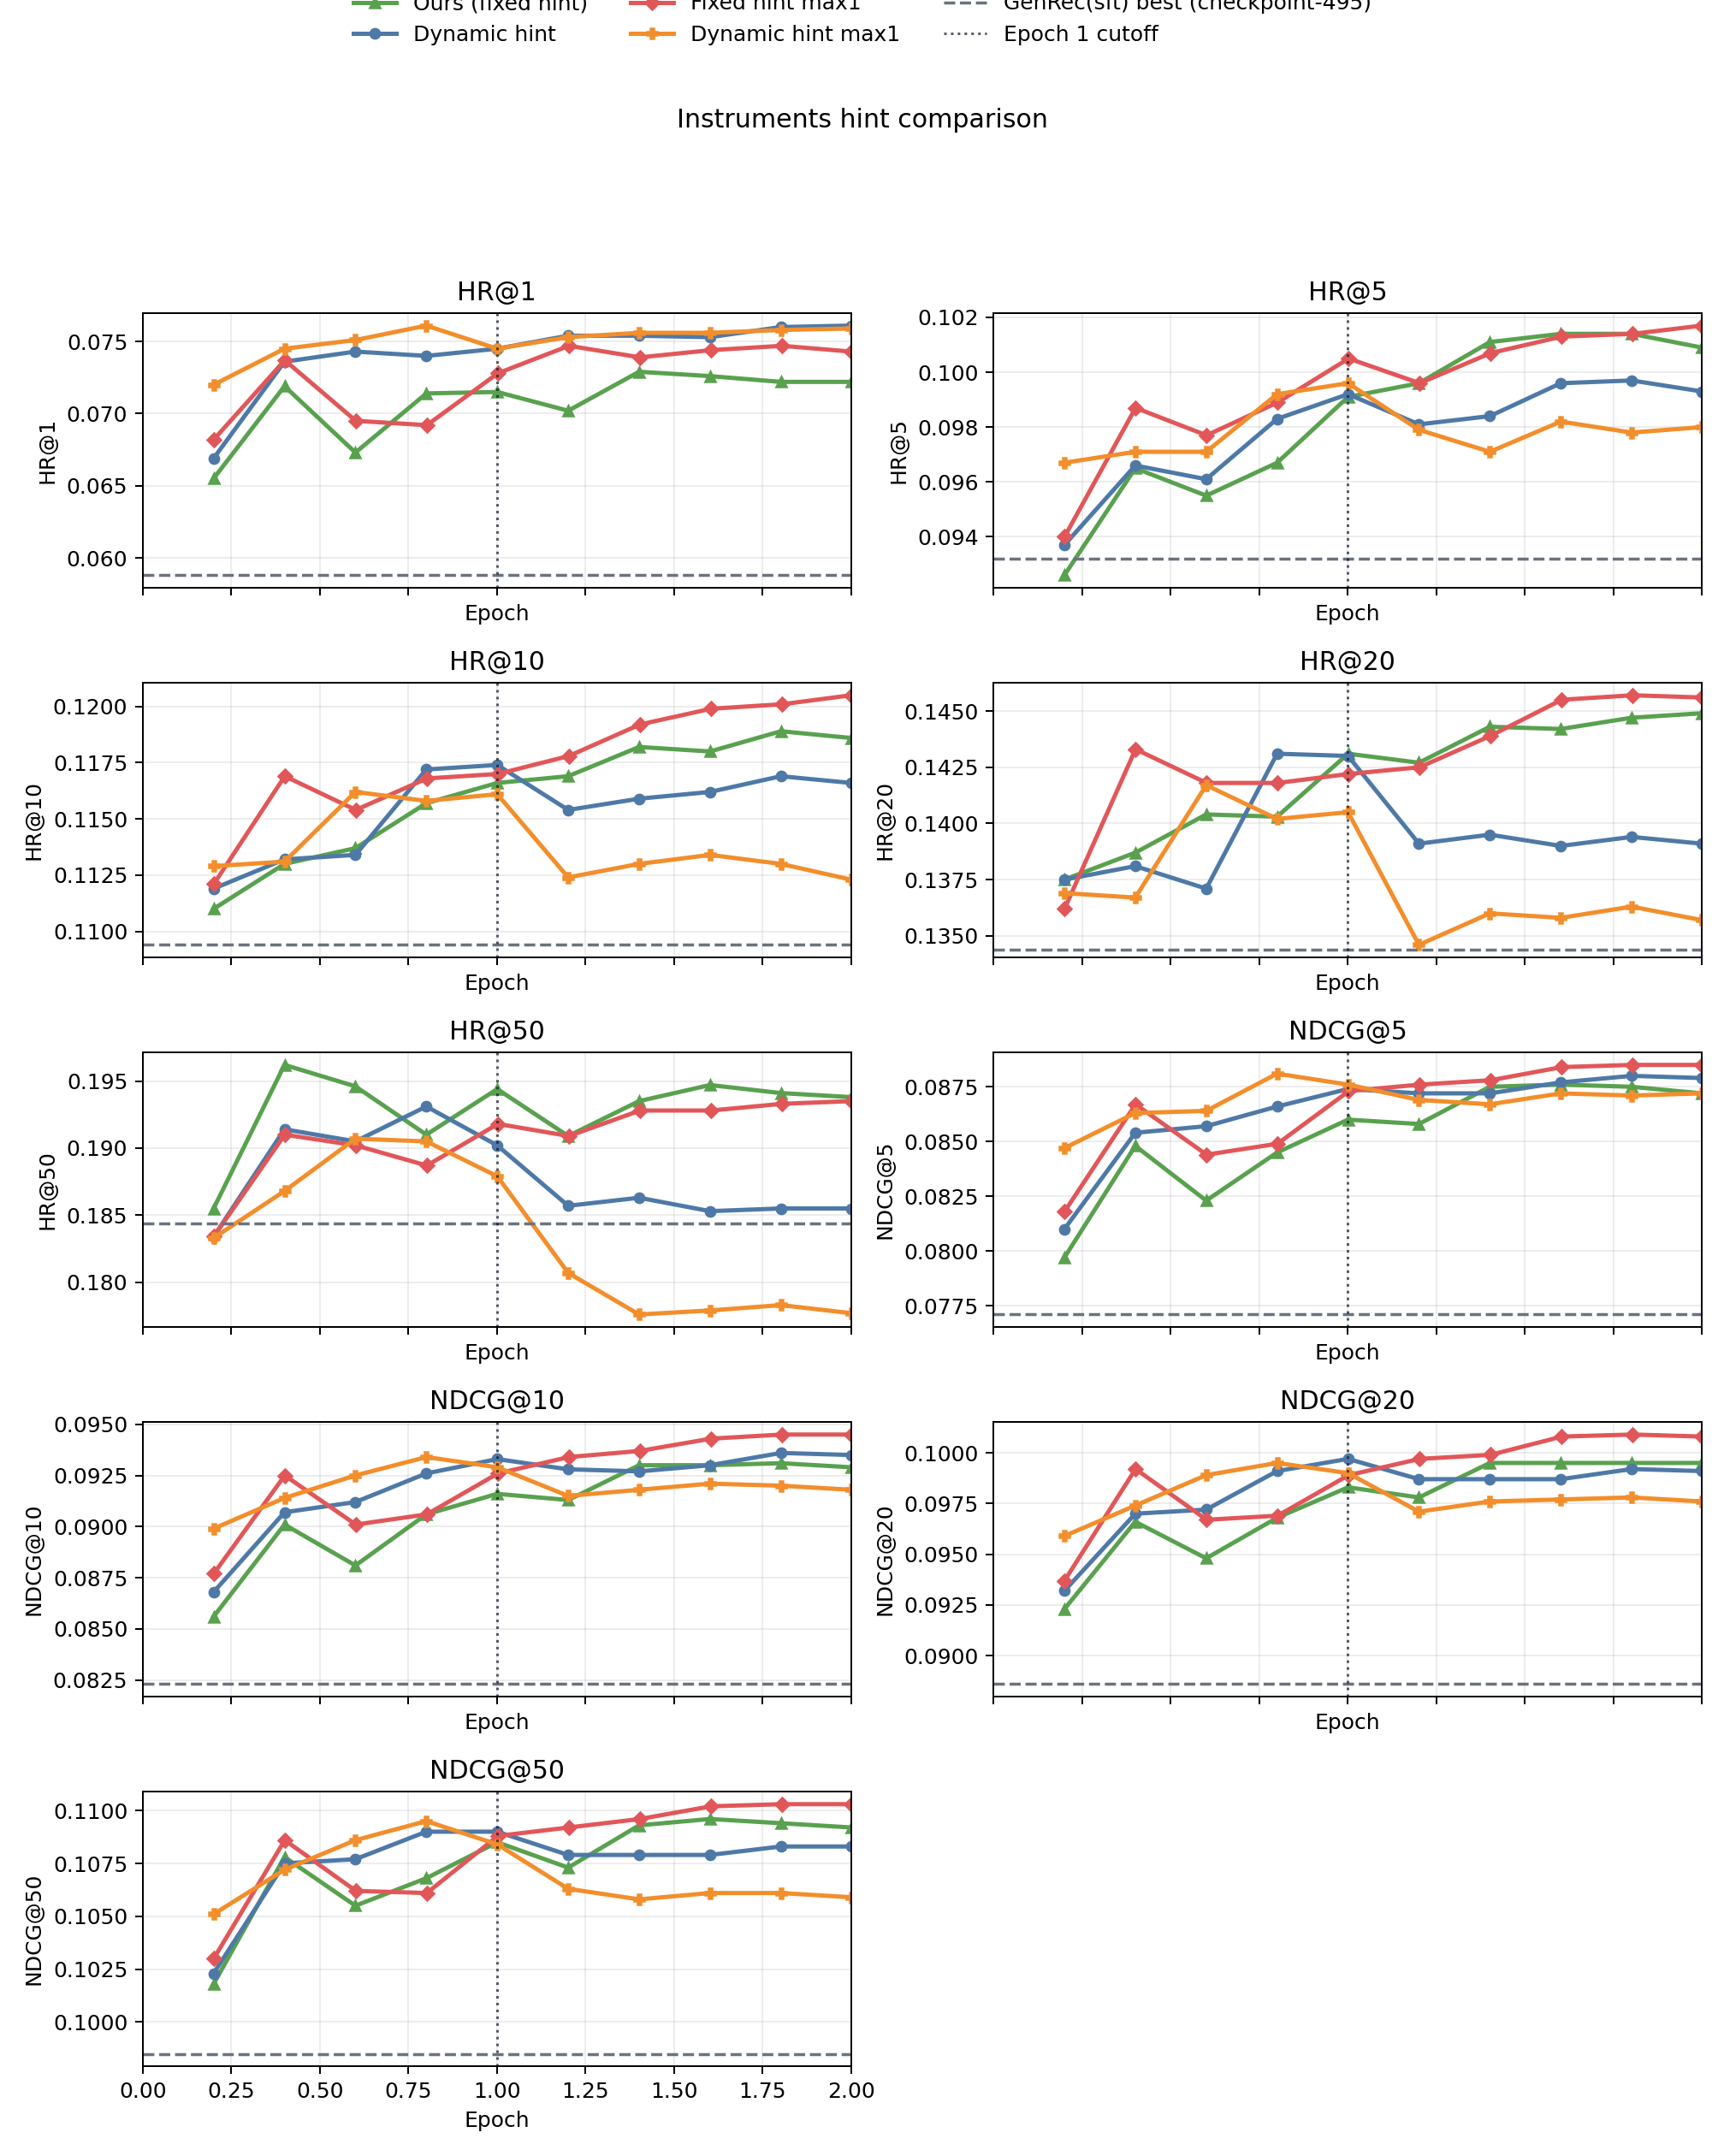
\includegraphics[width=\textwidth]{assets/genrec-only-instruments-hint-comparison-curves.png}
\caption{Instruments 上 \texttt{Ours(fixed hint)}、\texttt{dynamic hint}、\texttt{fixed hint max1} 与 \texttt{dynamic hint max1} 的完整曲线对比。图中统一展示 9 个指标；横轴统一使用 epoch，其中 full hint / dynamic 主线按 \texttt{3326 step = 2 epoch} 归一化，\texttt{fixed hint max1} 按 \texttt{2652 step = 2 epoch} 归一化。}
\label{fig:genrec-only-instruments-hint-comparison-curves}
\end{figure}

\section{RQ3: Ablation Study}

这一节把消融分成两层：训练任务范围，以及 loss 设计。前者只比较当前已经跑完的 three-way fixed prefix variants；后者则把 \texttt{fixed}、\texttt{fixed+CE} 和正在跑的 full-sequence 线并列放进同一张状态表。

\subsection{Training Task Scope}

当前已经落地的三档训练数据范围是：\texttt{Ours(3-task)}、\texttt{Fixed first-token hint}，以及当前仓库里实际已跑出的两任务变体 \texttt{Fixed(sid+title+desc)}。

\begin{table}[H]
\centering
\scriptsize
\setlength{\tabcolsep}{4pt}
\renewcommand{\arraystretch}{1.08}
\begin{tabular}{lccc}
\toprule
Metric & Fixed(taskfix) & Fixed(sid-only) & Fixed(sid+title+desc) \\
\midrule
HR@1 & 0.0722 & \underline{0.0743} & \textbf{0.0758} \\
HR@5 & \underline{0.1014} & \textbf{0.1017} & 0.1001 \\
HR@10 & \underline{0.1189} & \textbf{0.1205} & 0.1169 \\
HR@20 & \underline{0.1447} & \textbf{0.1456} & 0.1416 \\
HR@50 & \textbf{0.1941} & \underline{0.1935} & 0.1905 \\
NDCG@5 & \underline{0.0875} & \textbf{0.0885} & \textbf{0.0885} \\
NDCG@10 & 0.0931 & \textbf{0.0945} & \underline{0.0939} \\
NDCG@20 & 0.0995 & \textbf{0.1008} & \underline{0.1001} \\
NDCG@50 & 0.1094 & \textbf{0.1103} & \underline{0.1098} \\
\midrule
Selected ckpt & \texttt{checkpoint-2997} & \texttt{checkpoint-2652} & \texttt{checkpoint-3012} \\
\bottomrule
\end{tabular}
\caption{Instruments 上训练任务范围的 three-way ablation。}
\label{tab:genrec-only-rq3-task-scope}
\end{table}

\begin{figure}[p]
\centering
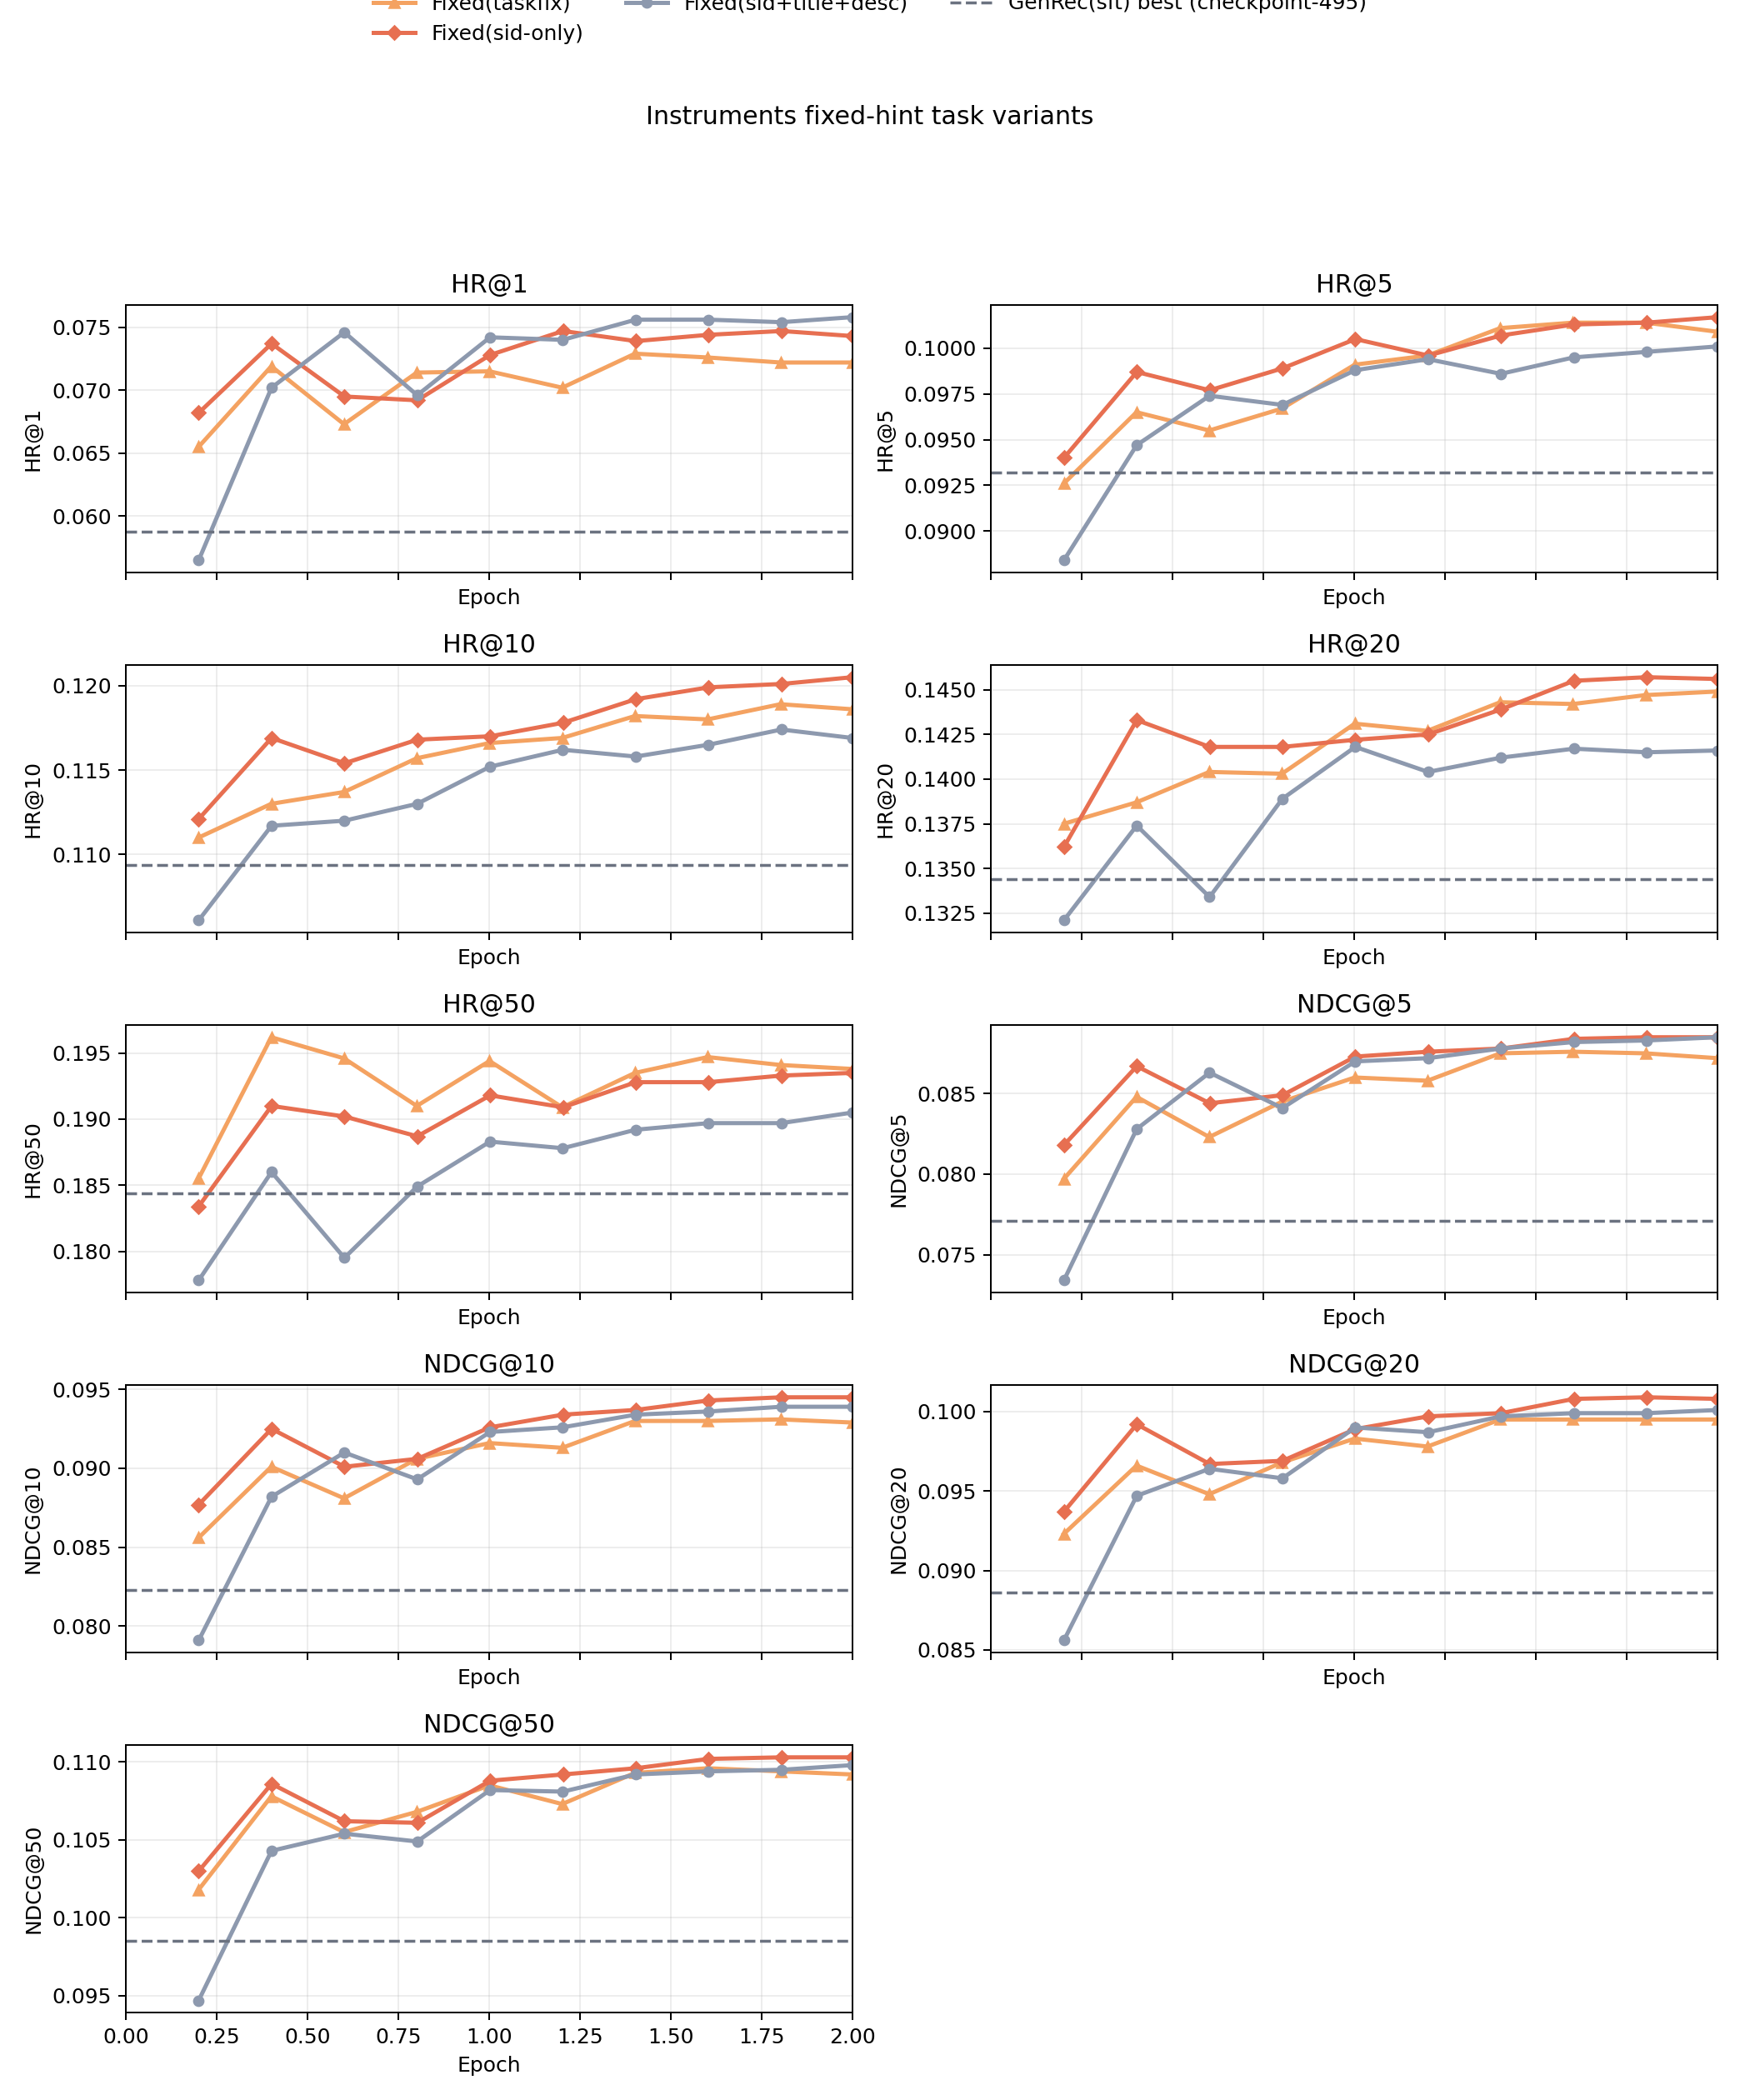
\includegraphics[width=\textwidth]{assets/genrec-only-instruments-fixed-task-variants-curves.png}
\caption{Instruments 上三个 fixed-hint taskfix 变体的完整 checkpoint 曲线。图中统一展示 9 个指标：\texttt{HR@1/5/10/20/50} 与 \texttt{NDCG@5/10/20/50}；横轴统一使用 epoch，并分别按 \texttt{3326 / 2652 / 3012 step = 2 epoch} 归一化；虚线表示 \texttt{GenRec(sft)} 的整体 best（\texttt{checkpoint-495}）。}
\label{fig:genrec-only-instruments-fixed-task-variants-curves}
\end{figure}

\subsection{Loss Design}

loss 层面的比较只保留三种口径：\texttt{suffix-only GRPO}、\texttt{prefix SFT + suffix-only GRPO}、以及 \texttt{Full-sequence SFT + GRPO}。

\begin{table}[H]
\centering
\scriptsize
\setlength{\tabcolsep}{4pt}
\renewcommand{\arraystretch}{1.08}
\resizebox{\textwidth}{!}{%
\begin{tabular}{lccc}
\toprule
Metric & Suffix-only GRPO & Prefix SFT + suffix-only GRPO & Full-sequence SFT + GRPO \\
\midrule
HR@1 & 0.0722 & 0.0764 & \textemdash \\
HR@5 & 0.1014 & 0.1009 & \textemdash \\
HR@10 & 0.1189 & 0.1180 & \textemdash \\
HR@20 & 0.1447 & 0.1435 & \textemdash \\
HR@50 & 0.1941 & 0.1985 & \textemdash \\
NDCG@5 & 0.0875 & 0.0890 & \textemdash \\
NDCG@10 & 0.0931 & 0.0945 & \textemdash \\
NDCG@20 & 0.0995 & 0.1009 & \textemdash \\
NDCG@50 & 0.1094 & 0.1118 & \textemdash \\
\midrule
Selected ckpt & \texttt{checkpoint-2997} & \texttt{checkpoint-1665} & \texttt{running} \\
\bottomrule
\end{tabular}
}
\caption{RQ3 中 loss 设计的当前状态表。}
\label{tab:genrec-only-rq3-loss-design}
\end{table}

当前 full-sequence 列仍在跑，对应 launcher：\texttt{hope/Instruments-genrec/rl\_fixed\_full\_sequence\_sft.sh}；已完成的 prefix-SFT 列这里使用 \texttt{CE=0.005} 作为代表性 fixed+CE readout。

\section{RQ4: CE Loss Influence}

这一节专门分析 fixed CE coefficient 对后训练结果的影响。正文只保留 \texttt{Instruments} 和 \texttt{Arts} 两个数据集上的 \texttt{0.001 / 0.005 / 0.01} sweep。

\subsection{Arts}

\begin{table}[H]
\centering
\scriptsize
\setlength{\tabcolsep}{4pt}
\renewcommand{\arraystretch}{1.08}
\begin{tabular}{lcccc}
\toprule
Metric & Fixed(no CE) & CE=0.001 & CE=0.005 & CE=0.01 \\
\midrule
HR@1 & \underline{0.0730} & 0.0710 & 0.0720 & \textbf{0.0734} \\
HR@5 & \underline{0.1041} & 0.1031 & \textbf{0.1048} & 0.1025 \\
HR@10 & \underline{0.1248} & 0.1244 & \textbf{0.1257} & 0.1216 \\
HR@20 & 0.1504 & \textbf{0.1537} & \underline{0.1518} & 0.1496 \\
HR@50 & \underline{0.2007} & \textbf{0.2029} & 0.2006 & 0.1978 \\
NDCG@5 & \textbf{0.0890} & 0.0874 & \underline{0.0889} & 0.0884 \\
NDCG@10 & \textbf{0.0956} & 0.0943 & \textbf{0.0956} & \underline{0.0946} \\
NDCG@20 & \textbf{0.1021} & \underline{0.1017} & \textbf{0.1021} & 0.1016 \\
NDCG@50 & \textbf{0.1120} & 0.1114 & \underline{0.1118} & 0.1111 \\
\midrule
Selected ckpt & \texttt{checkpoint-3368} & \texttt{checkpoint-2105} & \texttt{checkpoint-2105} & \texttt{checkpoint-4206} \\
\bottomrule
\end{tabular}
\caption{Arts 上 fixed CE 系数对比（含无 CE baseline）。}
\label{tab:genrec-only-arts-fixed-ce-coefficients}
\end{table}

\begin{figure}[p]
\centering
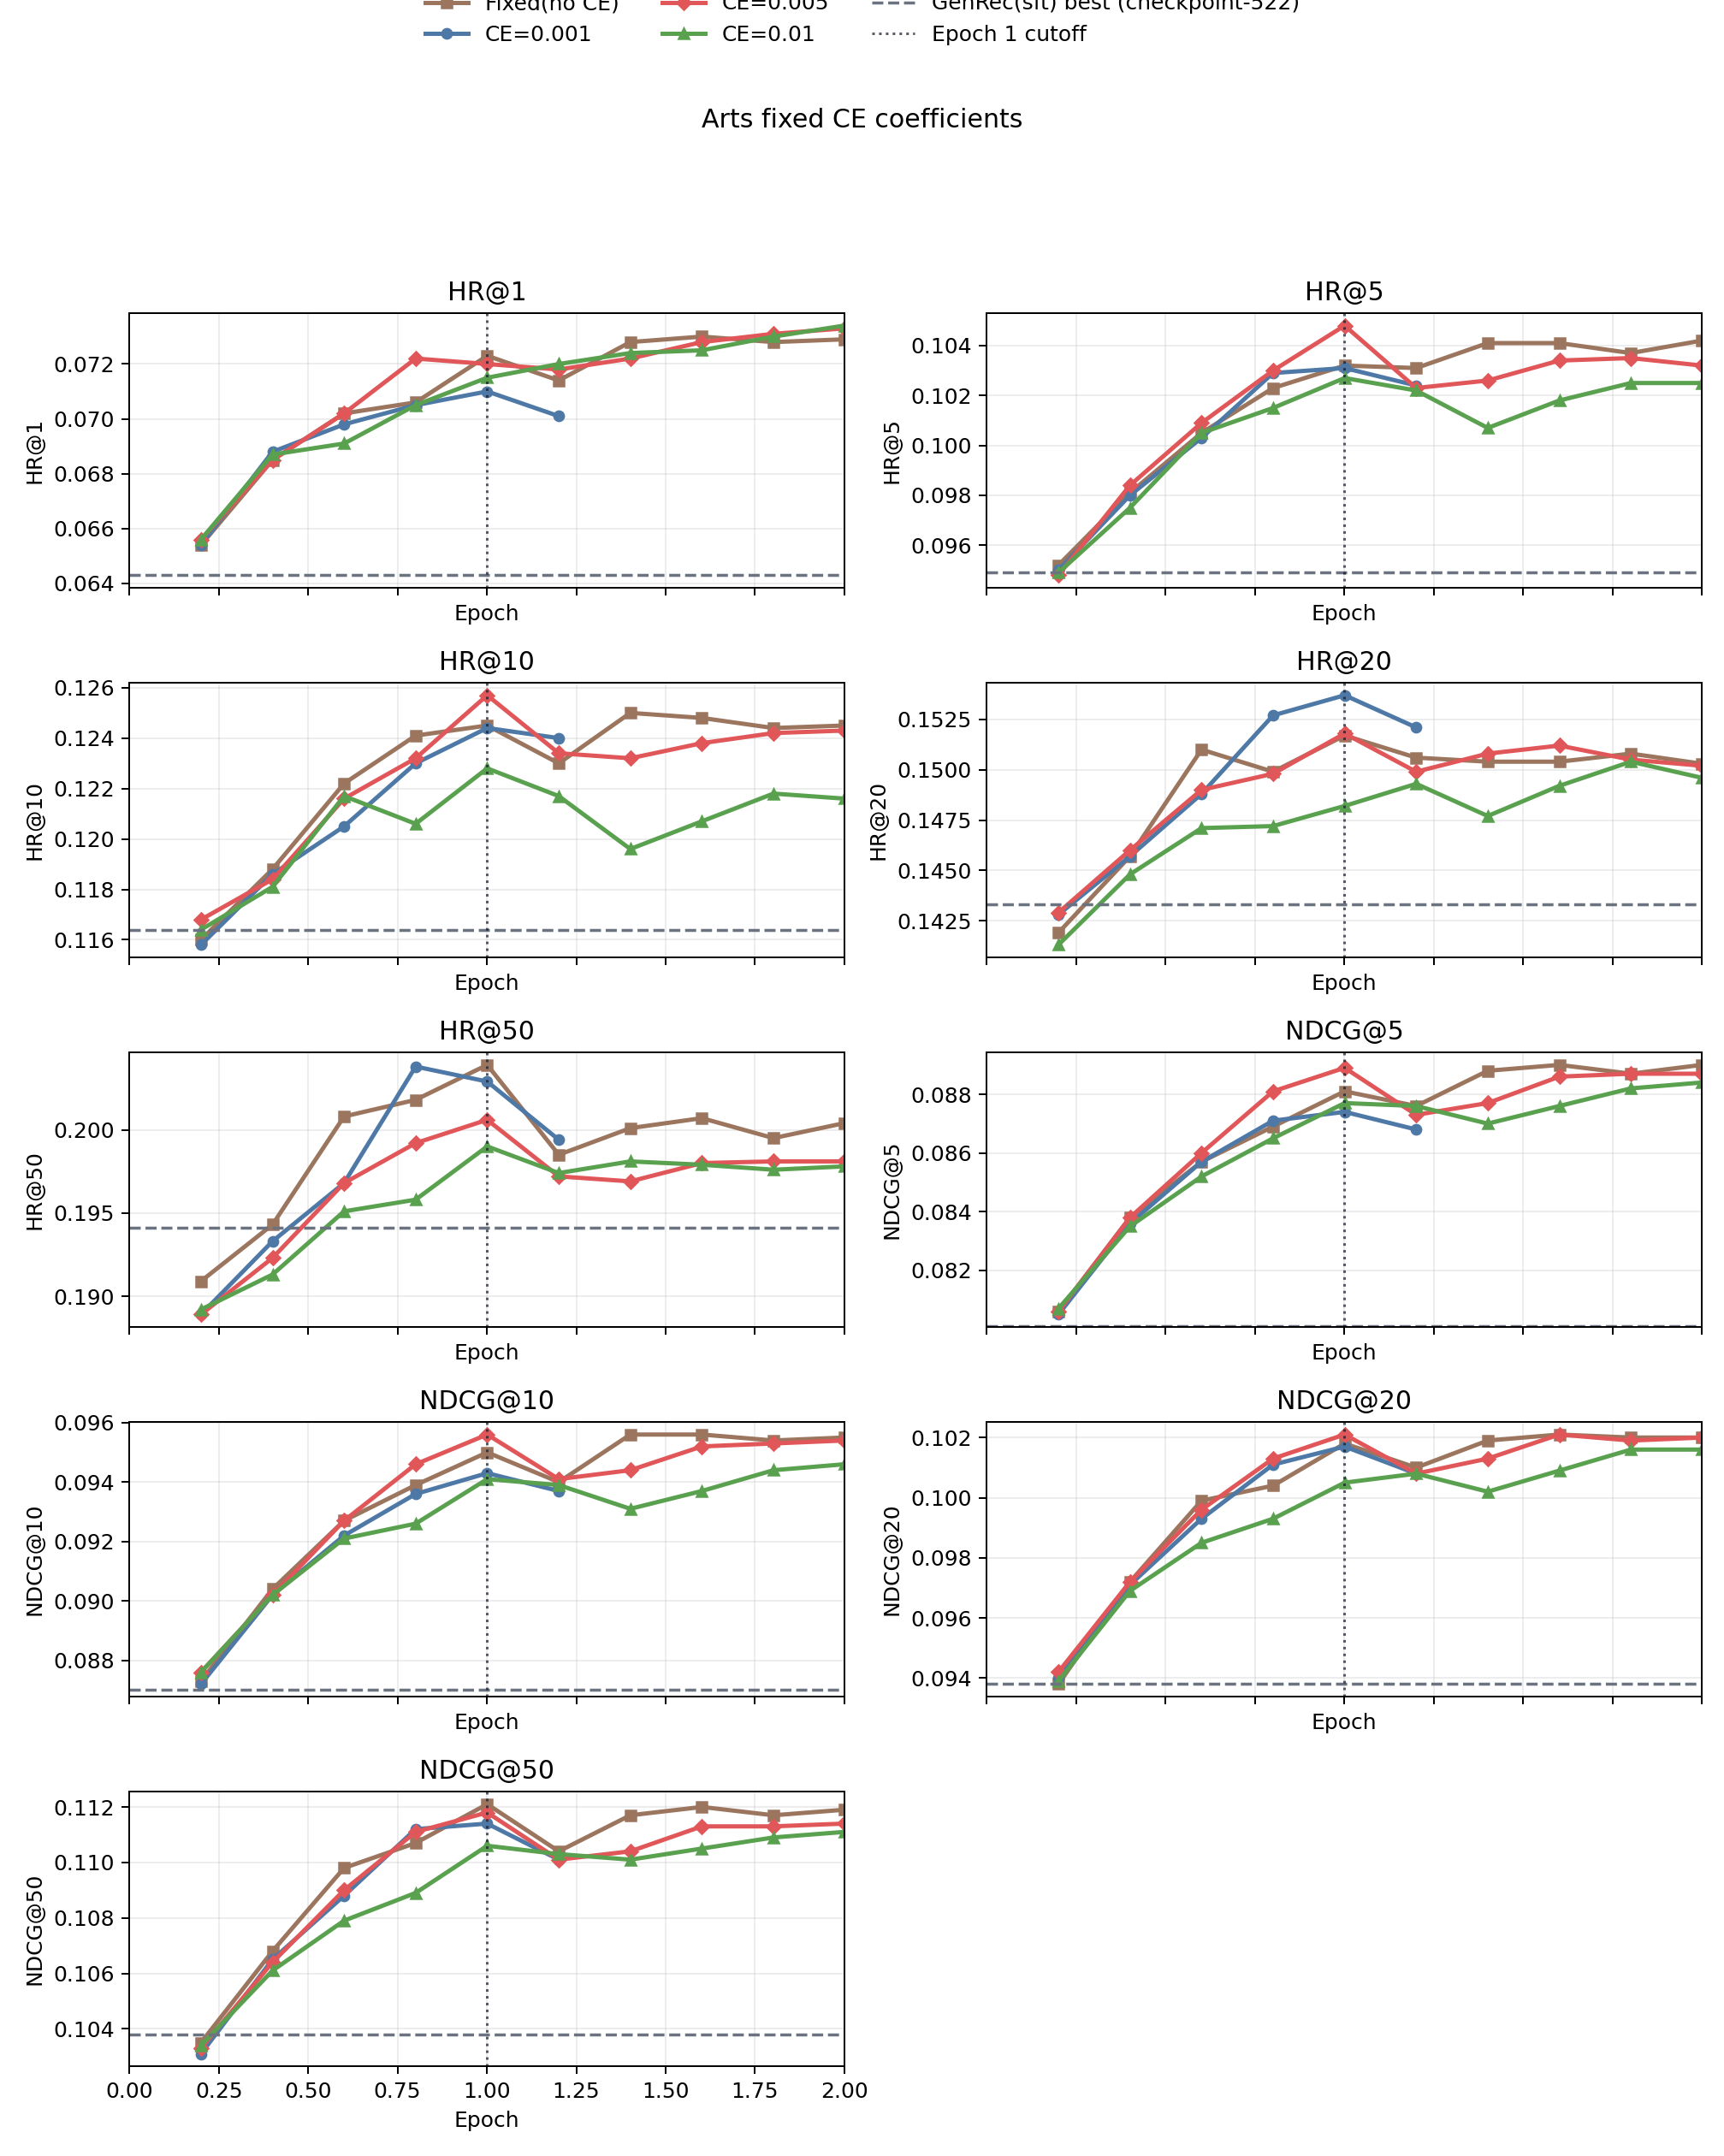
\includegraphics[width=\textwidth]{assets/genrec-only-arts-fixed-ce-coefficients-curves.png}
\caption{Arts 上 fixed CE 系数对比曲线。图中同时保留 \texttt{Fixed(no CE)} 基线，另外三条线分别对应 \texttt{CE=0.001 / 0.005 / 0.01}；横轴按 \texttt{4206 step = 2 epoch} 归一化；虚线表示 \texttt{GenRec(sft)} 的整体 best，竖向点线表示第一个 epoch 的 cutoff。}
\label{fig:genrec-only-arts-fixed-ce-coefficients-curves}
\end{figure}

\subsection{Instruments}

\begin{table}[H]
\centering
\scriptsize
\setlength{\tabcolsep}{4pt}
\renewcommand{\arraystretch}{1.08}
\begin{tabular}{lcccc}
\toprule
Metric & Fixed(no CE) & CE=0.001 & CE=0.005 & CE=0.01 \\
\midrule
HR@1 & 0.0722 & 0.0747 & \textbf{0.0764} & \underline{0.0761} \\
HR@5 & \underline{0.1014} & 0.0993 & 0.1009 & \textbf{0.1016} \\
HR@10 & \underline{0.1189} & 0.1168 & 0.1180 & \textbf{0.1204} \\
HR@20 & 0.1447 & \underline{0.1449} & 0.1435 & \textbf{0.1456} \\
HR@50 & 0.1941 & \underline{0.1951} & \textbf{0.1985} & 0.1943 \\
NDCG@5 & 0.0875 & 0.0875 & \underline{0.0890} & \textbf{0.0893} \\
NDCG@10 & 0.0931 & 0.0931 & \underline{0.0945} & \textbf{0.0953} \\
NDCG@20 & 0.0995 & 0.1002 & \underline{0.1009} & \textbf{0.1016} \\
NDCG@50 & 0.1094 & 0.1102 & \textbf{0.1118} & \underline{0.1113} \\
\midrule
Selected ckpt & \texttt{checkpoint-2997} & \texttt{checkpoint-2664} & \texttt{checkpoint-1665} & \texttt{checkpoint-2997} \\
\bottomrule
\end{tabular}
\caption{Instruments 上 fixed-hint CE 系数对比（含无 CE baseline）。}
\label{tab:genrec-only-instruments-fixed-ce-coefficients}
\end{table}

\begin{figure}[p]
\centering
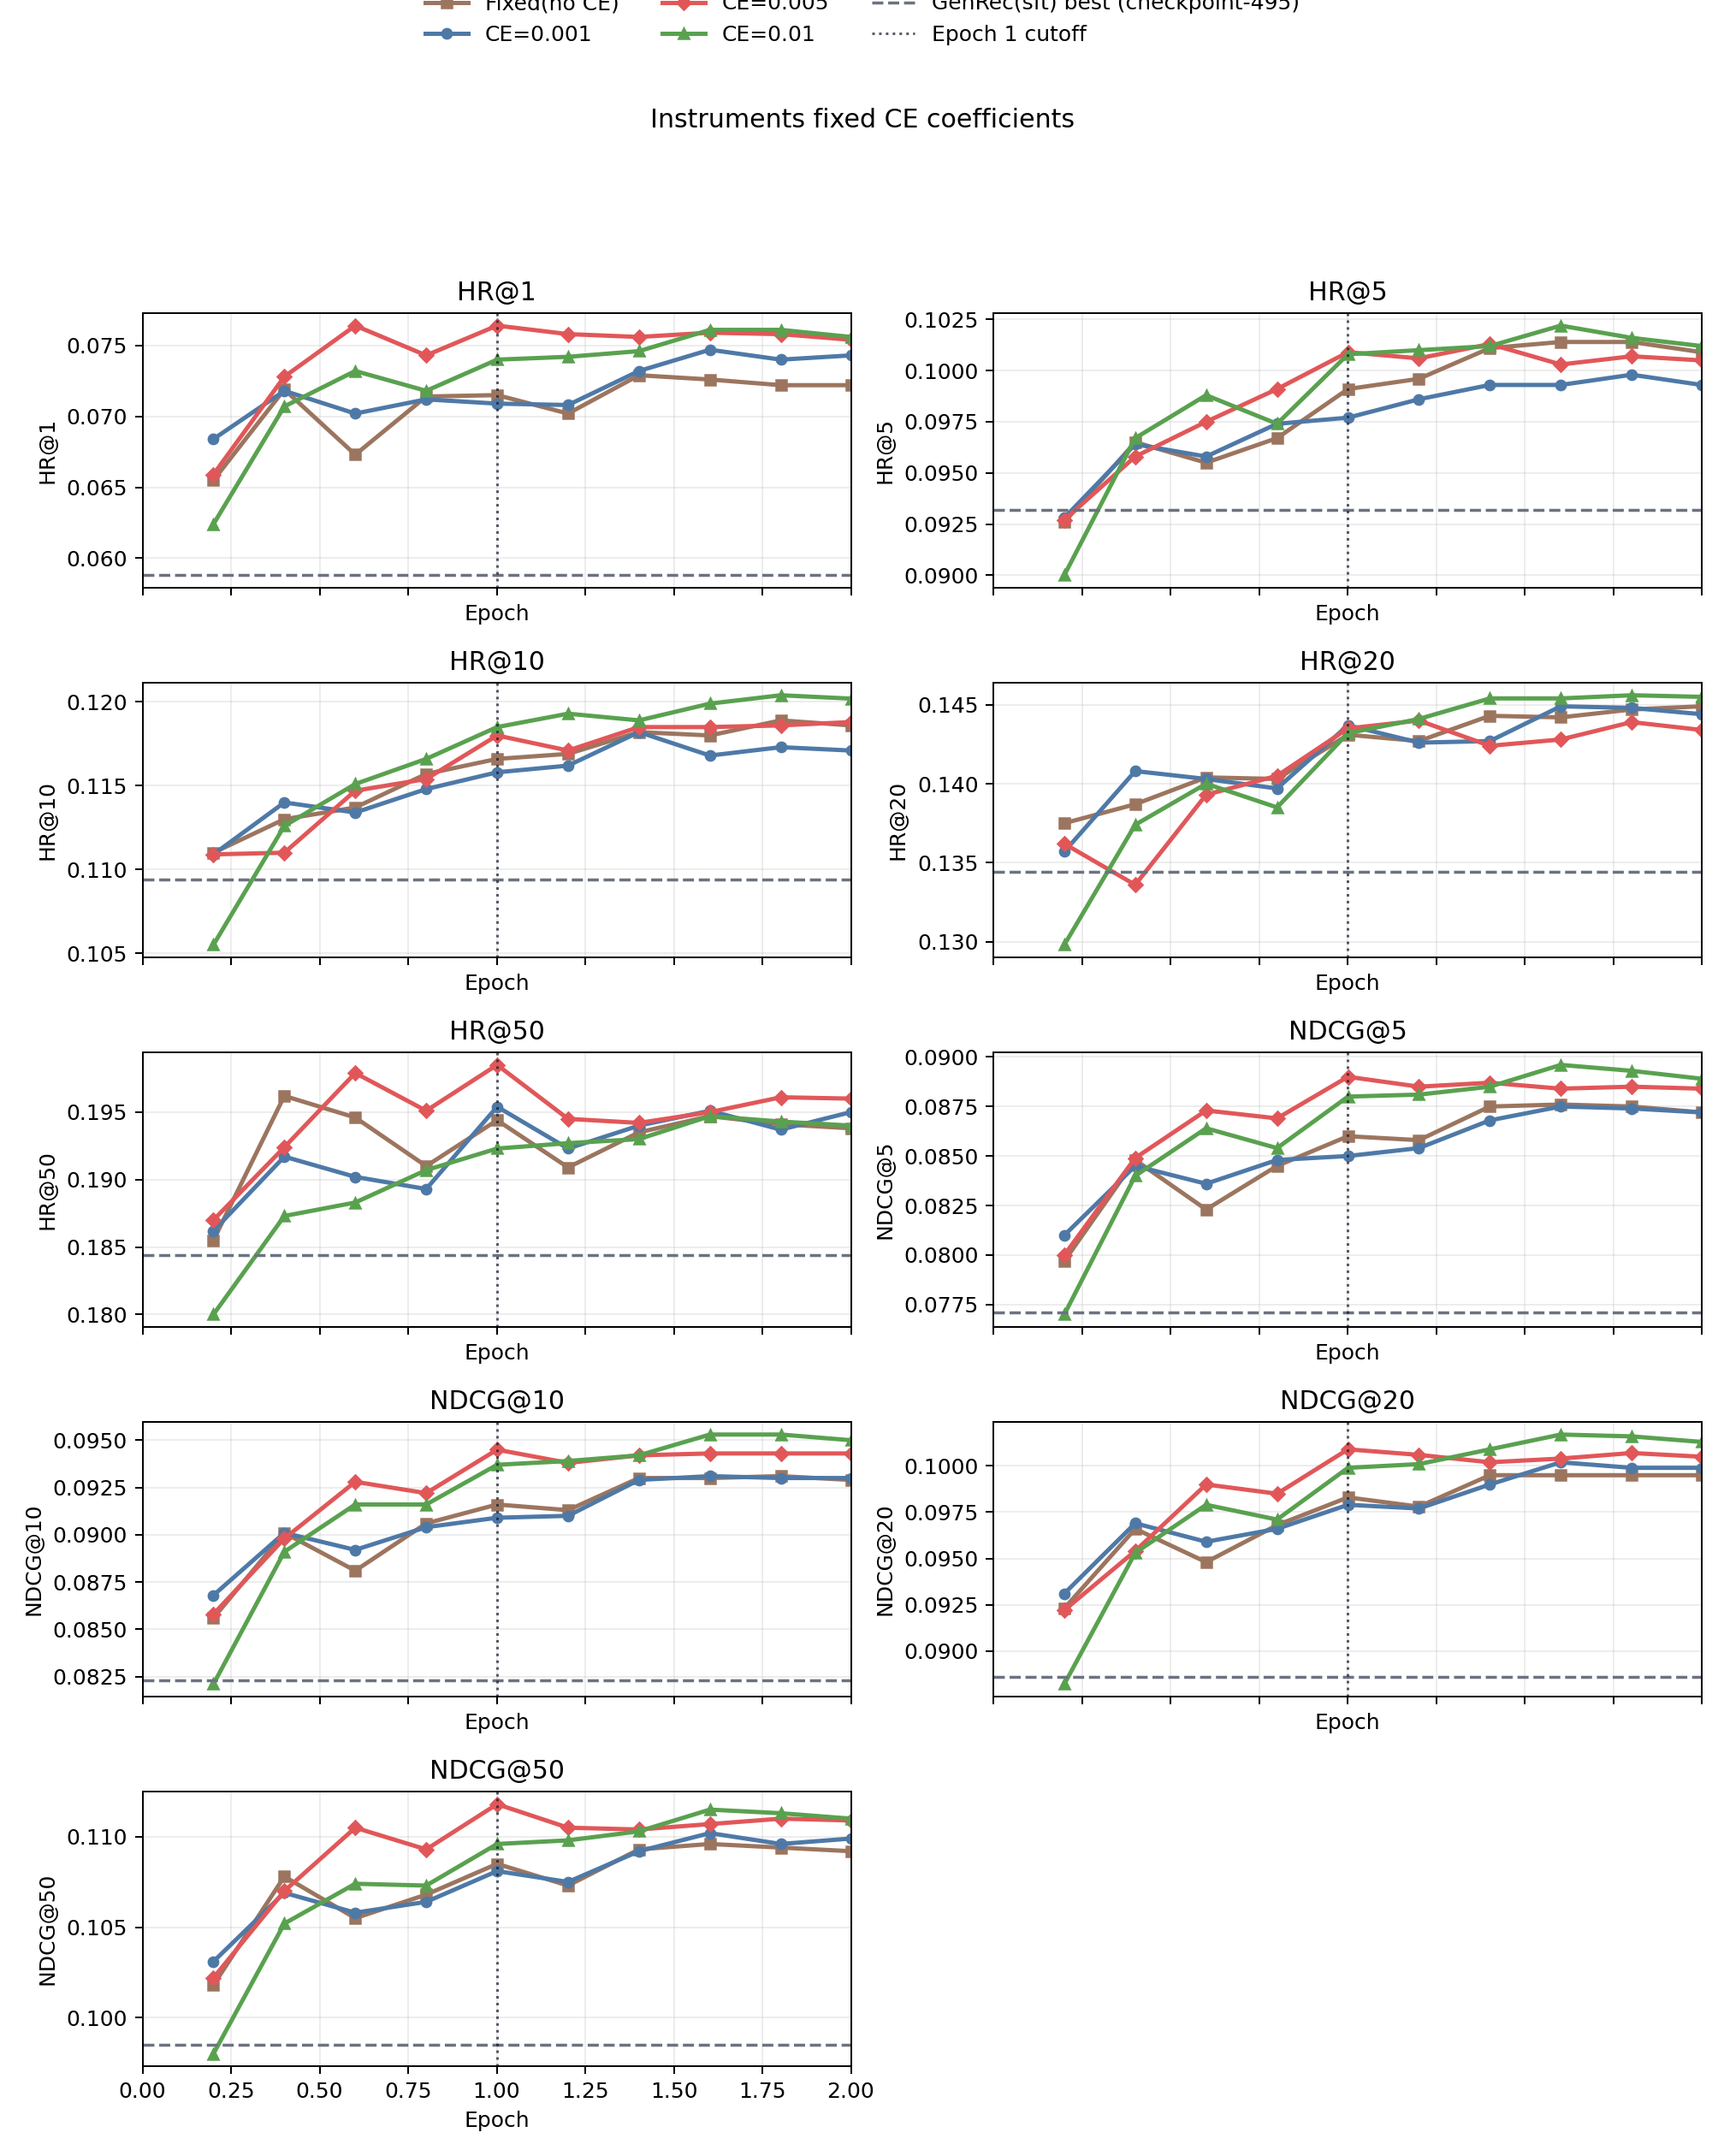
\includegraphics[width=\textwidth]{assets/genrec-only-instruments-fixed-ce-coefficients-curves.png}
\caption{Instruments 上 fixed-hint CE 系数对比曲线。图中同时保留 \texttt{Fixed(no CE)} 基线，另外三条线分别对应 \texttt{CE=0.001 / 0.005 / 0.01}；横轴按 \texttt{3326 step = 2 epoch} 归一化；虚线表示 \texttt{GenRec(sft)} 的整体 best，竖向点线表示第一个 epoch 的 cutoff。}
\label{fig:genrec-only-instruments-fixed-ce-coefficients-curves}
\end{figure}

\subsection{Cross-Dataset Summary}

\begin{table}[H]
\centering
\scriptsize
\setlength{\tabcolsep}{4pt}
\renewcommand{\arraystretch}{1.08}
\begin{tabular}{p{2.0cm} p{3.0cm} p{3.0cm} p{5.0cm}}
\toprule
Dataset & Best top-10 coefficient & Best coverage coefficient & Reading \\
\midrule
Instruments & \texttt{CE=0.01} & \texttt{CE=0.005} & 大系数继续抬高 long-run top-10，但 coverage 峰值仍出现在中档系数 \\
Arts & \texttt{CE=0.005} / no-CE tie & \texttt{CE=0.001} & 小系数更像 mild coverage regularizer，\texttt{CE=0.01} 没有复制 Instruments 的 top-10 收益 \\
\bottomrule
\end{tabular}
\caption{RQ4 的跨数据集 summary。}
\label{tab:genrec-only-rq4-cross-dataset-summary}
\end{table}

\clearpage
\appendix

\section{Supplementary Full Curves}

这一节保留完整 checkpoint 曲线，作为 RQ1--RQ4 正文之外的补充证据。 Instruments、Games 与 Arts 都保留 RL 全轨迹并标出 first-epoch 边界； 各图中的虚线统一表示 \texttt{GenRec(sft)} 的整体 best。

\subsection{Instruments}

\begin{figure}[p]
\centering

\includegraphics[width=\textwidth]{assets/genrec-only-instruments-curves.png}
\caption{Instruments 上 GenRec RL 变体的完整 checkpoint 曲线。图中统一展示 9 个指标：\texttt{HR@1/5/10/20/50} 与 \texttt{NDCG@5/10/20/50}；横轴按 Instruments RL 主线的 \texttt{3326 step = 2 epoch} 归一化；虚线表示 \texttt{GenRec(sft)} 的整体 best，竖向点线表示第一个 epoch 的 cutoff（\texttt{step <= 1663}）。}
\label{fig:genrec-only-instruments-curves}
\end{figure}

\subsection{Games}

\begin{figure}[p]
\centering
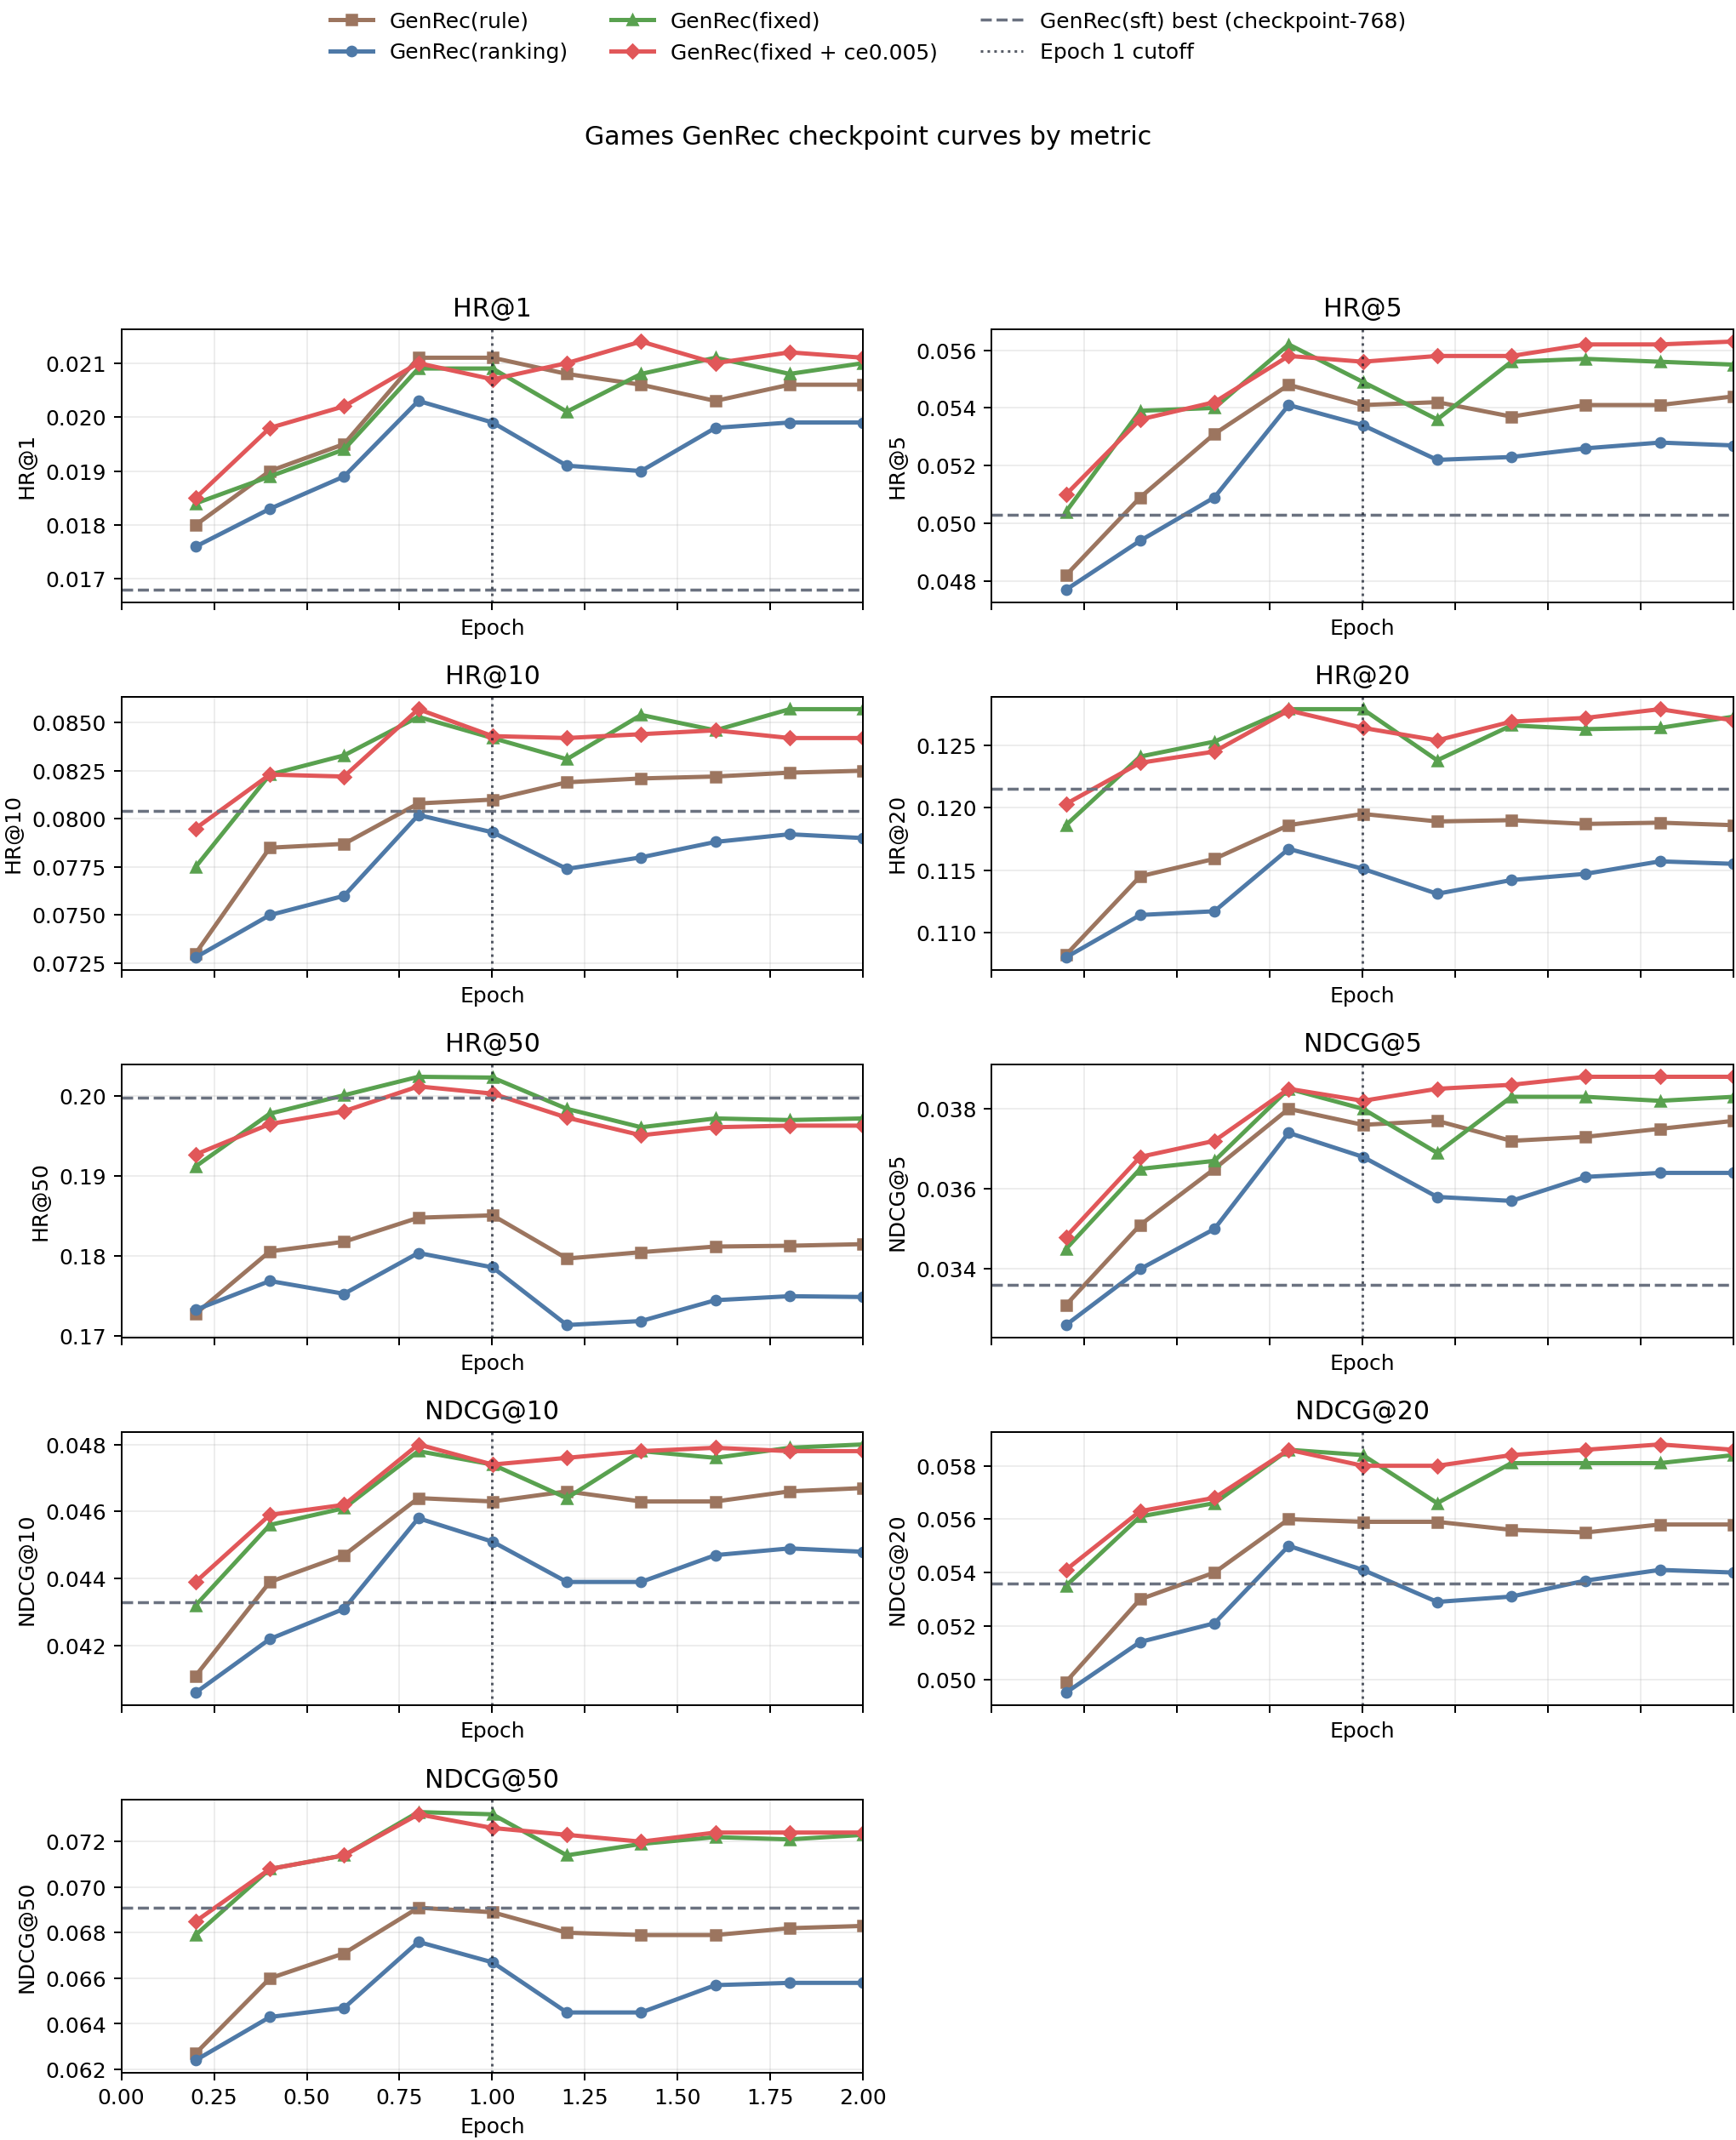
\includegraphics[width=\textwidth]{assets/genrec-only-games-curves.png}
\caption{Games 上 GenRec RL 变体的完整 checkpoint 曲线。图中统一展示 9 个指标：\texttt{HR@1/5/10/20/50} 与 \texttt{NDCG@5/10/20/50}；横轴按 Games RL 主线的 \texttt{8752 step = 2 epoch} 归一化；虚线表示 \texttt{GenRec(sft)} 的整体 best，竖向点线表示第一个 epoch 的 cutoff（\texttt{step <= 4376}）。}
\label{fig:genrec-only-games-curves}
\end{figure}

\subsection{Arts}

\begin{figure}[p]
\centering
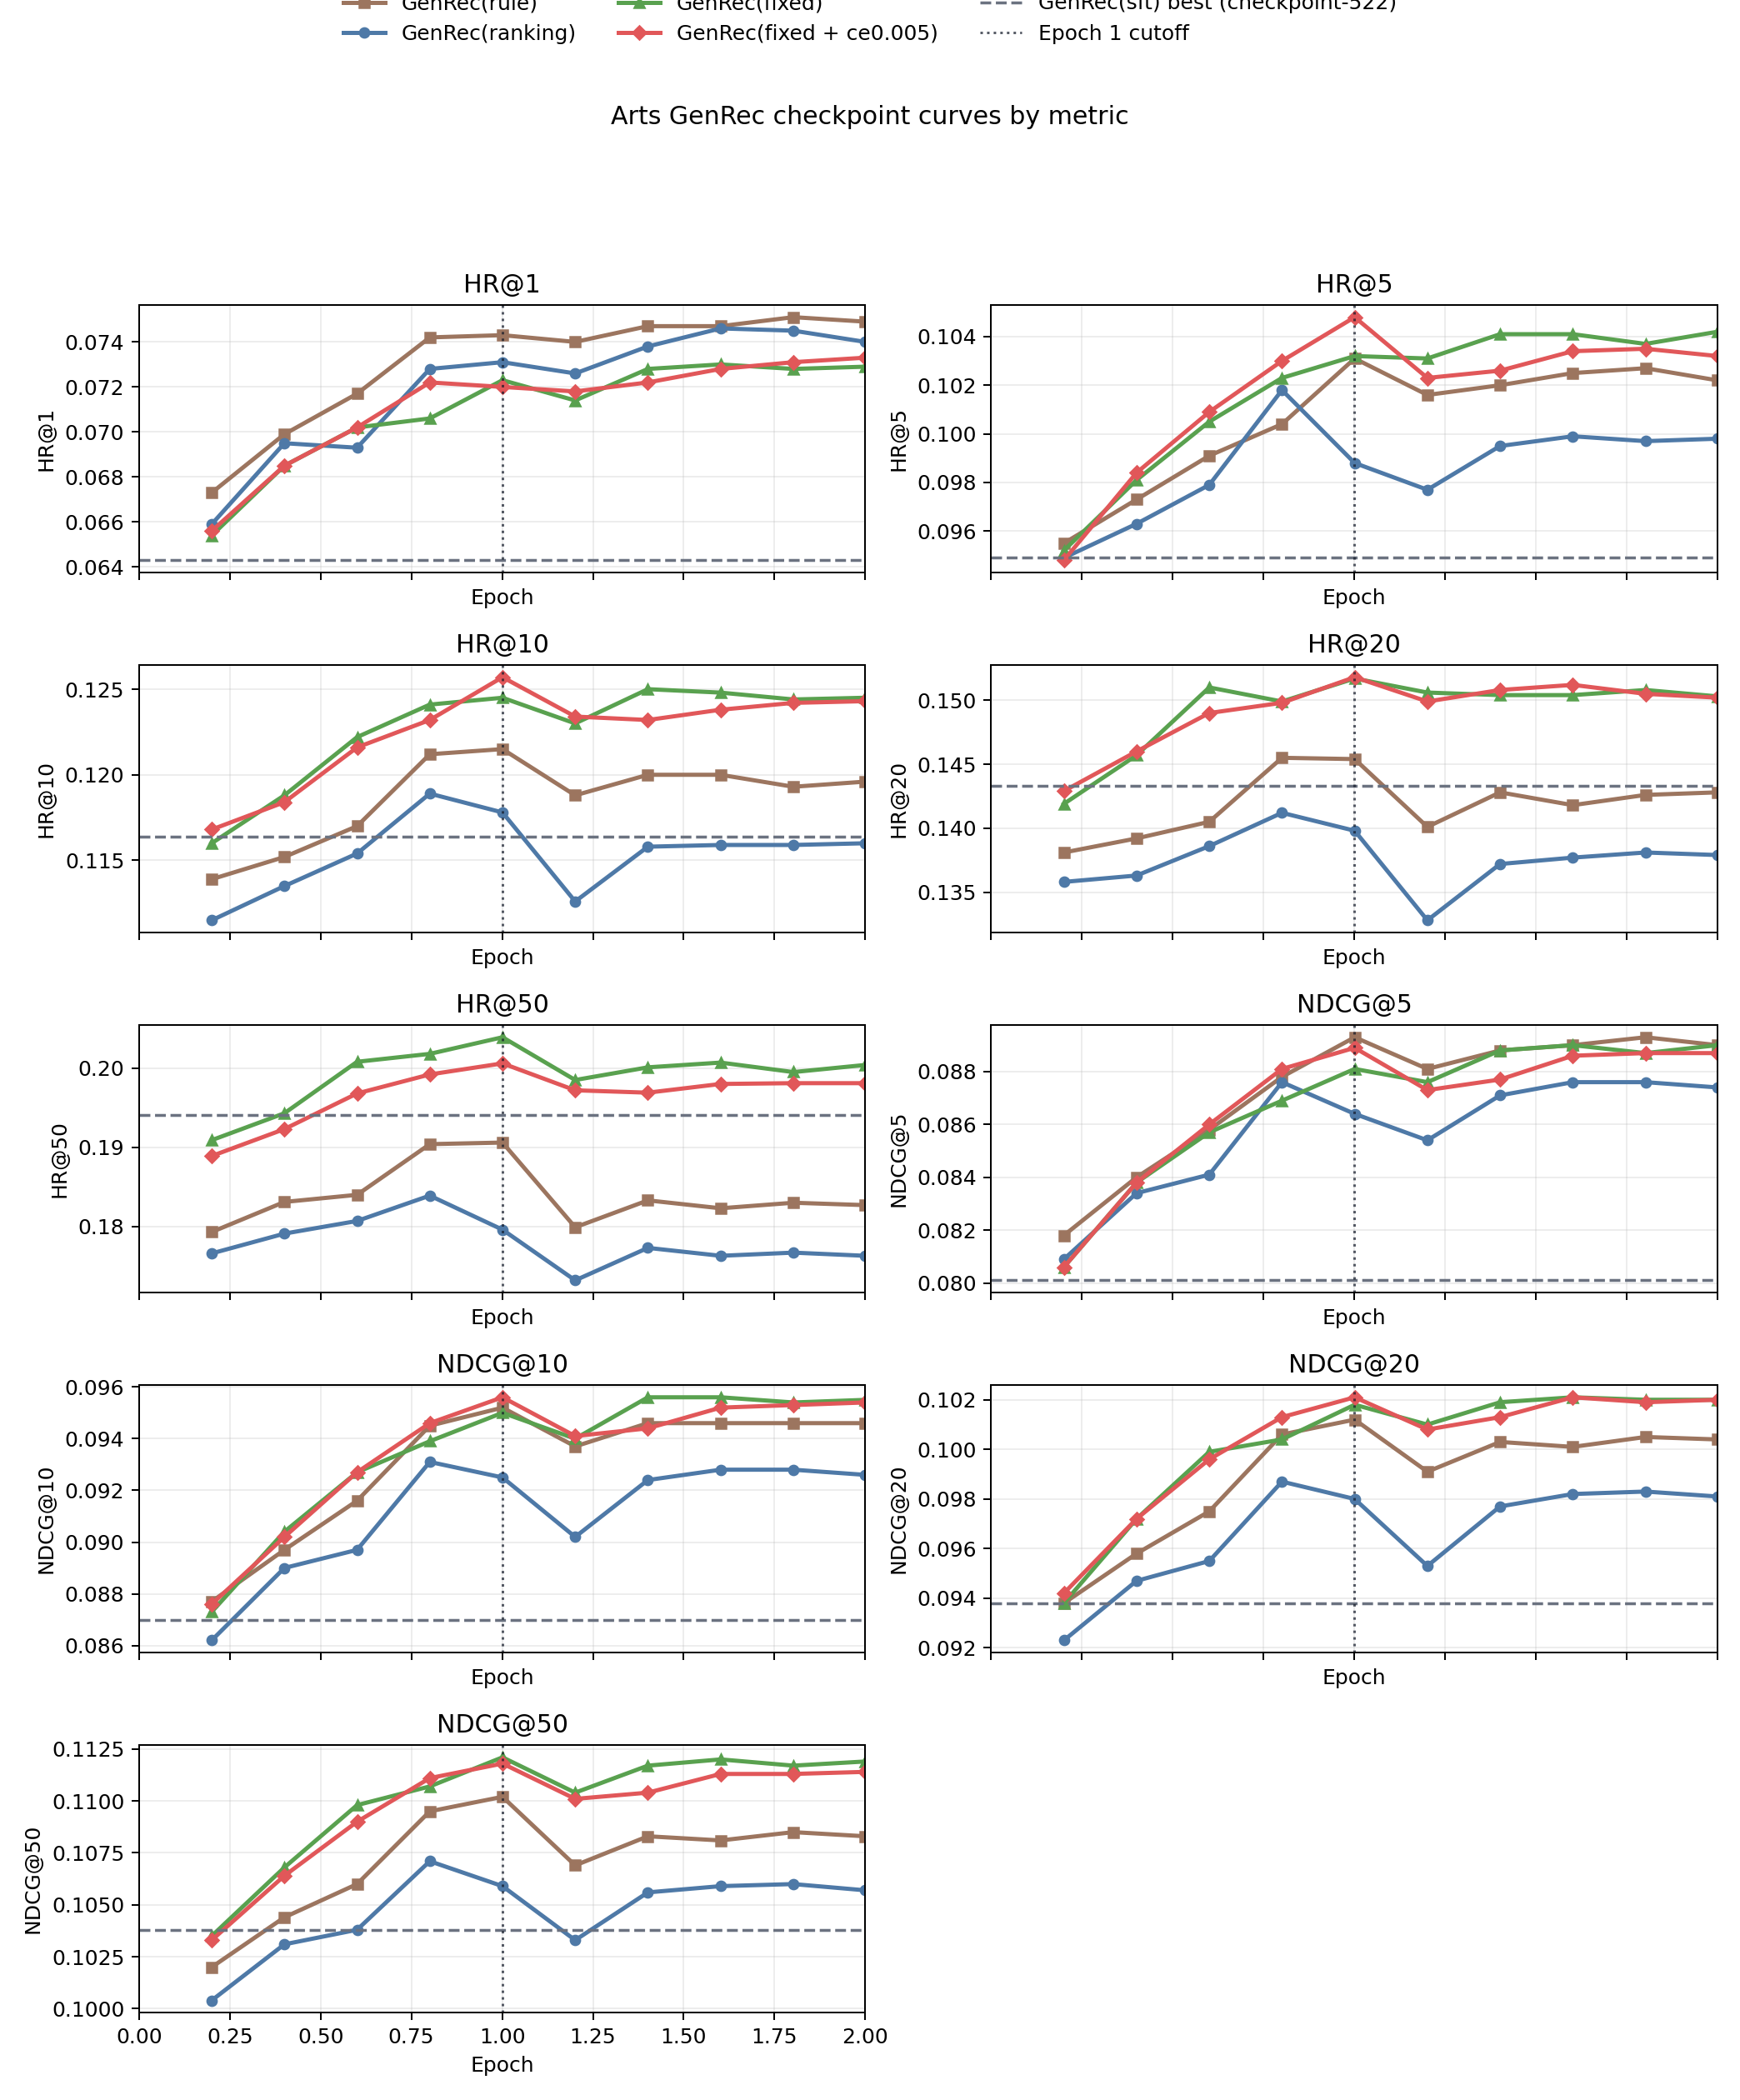
\includegraphics[width=\textwidth]{assets/genrec-only-arts-curves.png}
\caption{Arts 上 GenRec RL 变体的完整 checkpoint 曲线。图中统一展示 9 个指标：\texttt{HR@1/5/10/20/50} 与 \texttt{NDCG@5/10/20/50}；横轴按 Arts RL 主线的 \texttt{4206 step = 2 epoch} 归一化；虚线表示 \texttt{GenRec(sft)} 的整体 best，竖向点线表示第一个 epoch 的 cutoff（\texttt{step <= 2103}）。}
\label{fig:genrec-only-arts-curves}
\end{figure}

\section{RL First-Epoch Best}

这一节只对 RL 变体收紧选点范围： Instruments 的 RL 列只在 \texttt{checkpoint step <= 1663} 内选 best； Games 的 RL 列只在 \texttt{checkpoint step <= 4376} 内选 best； Arts 的 RL 列只在 \texttt{checkpoint step <= 2103} 内选 best； 非 RL 的 \texttt{GenRec(sft)} 仍保持其整体 best。 每个变体一旦按 \texttt{NDCG@10} 选出 checkpoint，整行指标与最后一行列出的 \texttt{ckpt} 都固定来自这个同一个 checkpoint。

\subsection{Instruments}

\begin{table}[H]
\centering
\scriptsize
\setlength{\tabcolsep}{4pt}
\renewcommand{\arraystretch}{1.08}
\resizebox{\textwidth}{!}{%
\begin{tabular}{lccccc}
\toprule
Metric & GenRec(sft) & GenRec(rule) & GenRec(ranking) & GenRec(fixed) & GenRec(fixed + ce0.005) \\
\midrule
HR@1 & 0.0588 & \underline{0.0778} & \textbf{0.0794} & 0.0714 & 0.0764 \\
HR@5 & 0.0932 & \textbf{0.1004} & \underline{0.0983} & 0.0967 & 0.0975 \\
HR@10 & 0.1094 & \textbf{0.1158} & 0.1128 & \underline{0.1157} & 0.1147 \\
HR@20 & 0.1344 & 0.1372 & 0.1344 & \textbf{0.1403} & \underline{0.1393} \\
HR@50 & 0.1844 & 0.1754 & 0.1723 & \underline{0.1910} & \textbf{0.1979} \\
NDCG@5 & 0.0771 & \textbf{0.0896} & \underline{0.0891} & 0.0845 & 0.0873 \\
NDCG@10 & 0.0823 & \textbf{0.0945} & \underline{0.0938} & 0.0906 & 0.0928 \\
NDCG@20 & 0.0886 & \textbf{0.0999} & \underline{0.0992} & 0.0968 & 0.0990 \\
NDCG@50 & 0.0985 & \underline{0.1075} & 0.1067 & 0.1068 & \textbf{0.1105} \\
\midrule
Selected ckpt & \texttt{checkpoint-495} & \texttt{checkpoint-1332} & \texttt{checkpoint-999} & \texttt{checkpoint-1332} & \texttt{checkpoint-999} \\
\bottomrule
\end{tabular}%
}
\caption{Instruments 上仅保留 GenRec 系列方法的结果。（RL 列仅在第一个 epoch 内按 \texttt{NDCG@10} 选 best）。}
\label{tab:genrec-only-instruments-rl-first-epoch}
\end{table}

\subsection{Games}

\begin{table}[H]
\centering
\scriptsize
\setlength{\tabcolsep}{4pt}
\renewcommand{\arraystretch}{1.08}
\resizebox{\textwidth}{!}{%
\begin{tabular}{lccccc}
\toprule
Metric & GenRec(sft) & GenRec(rule) & GenRec(ranking) & GenRec(fixed) & GenRec(fixed + ce0.005) \\
\midrule
HR@1 & 0.0168 & \textbf{0.0211} & 0.0203 & 0.0209 & \underline{0.0210} \\
HR@5 & 0.0503 & 0.0548 & 0.0541 & \textbf{0.0562} & \underline{0.0558} \\
HR@10 & 0.0804 & 0.0808 & 0.0802 & \underline{0.0853} & \textbf{0.0857} \\
HR@20 & 0.1215 & 0.1186 & 0.1167 & \textbf{0.1279} & \underline{0.1278} \\
HR@50 & 0.1998 & 0.1848 & 0.1804 & \textbf{0.2024} & \underline{0.2012} \\
NDCG@5 & 0.0336 & \underline{0.0380} & 0.0374 & \textbf{0.0385} & \textbf{0.0385} \\
NDCG@10 & 0.0433 & 0.0464 & 0.0458 & \underline{0.0478} & \textbf{0.0480} \\
NDCG@20 & 0.0536 & \underline{0.0560} & 0.0550 & \textbf{0.0586} & \textbf{0.0586} \\
NDCG@50 & 0.0691 & 0.0691 & 0.0676 & \textbf{0.0733} & \underline{0.0732} \\
\midrule
Selected ckpt & \texttt{checkpoint-768} & \texttt{checkpoint-3504} & \texttt{checkpoint-3504} & \texttt{checkpoint-3504} & \texttt{checkpoint-3504} \\
\bottomrule
\end{tabular}%
}
\caption{Games 上当前已测到的 GenRec 系列结果。（RL 列仅在第一个 epoch 内按 \texttt{NDCG@10} 选 best）。}
\label{tab:genrec-only-games-rl-first-epoch}
\end{table}

\subsection{Arts}

\begin{table}[H]
\centering
\scriptsize
\setlength{\tabcolsep}{4pt}
\renewcommand{\arraystretch}{1.08}
\resizebox{\textwidth}{!}{%
\begin{tabular}{lccccc}
\toprule
Metric & GenRec(sft) & GenRec(rule) & GenRec(ranking) & GenRec(fixed) & GenRec(fixed + ce0.005) \\
\midrule
HR@1 & 0.0643 & \textbf{0.0742} & \underline{0.0728} & 0.0706 & 0.0722 \\
HR@5 & 0.0949 & 0.1004 & 0.1018 & \underline{0.1023} & \textbf{0.1030} \\
HR@10 & 0.1164 & 0.1212 & 0.1189 & \textbf{0.1241} & \underline{0.1232} \\
HR@20 & 0.1433 & 0.1455 & 0.1412 & \textbf{0.1499} & \underline{0.1498} \\
HR@50 & 0.1941 & 0.1904 & 0.1839 & \textbf{0.2018} & \underline{0.1992} \\
NDCG@5 & 0.0801 & \underline{0.0878} & 0.0876 & 0.0869 & \textbf{0.0881} \\
NDCG@10 & 0.0870 & \underline{0.0945} & 0.0931 & 0.0939 & \textbf{0.0946} \\
NDCG@20 & 0.0938 & \underline{0.1006} & 0.0987 & 0.1004 & \textbf{0.1013} \\
NDCG@50 & 0.1038 & 0.1095 & 0.1071 & \underline{0.1107} & \textbf{0.1111} \\
\midrule
Selected ckpt & \texttt{checkpoint-522} & \texttt{checkpoint-1684} & \texttt{checkpoint-1684} & \texttt{checkpoint-1684} & \texttt{checkpoint-1684} \\
\bottomrule
\end{tabular}%
}
\caption{Arts 上当前已测到的 GenRec 系列结果。（RL 列仅在第一个 epoch 内按 \texttt{NDCG@10} 选 best）。}
\label{tab:genrec-only-arts-rl-first-epoch}
\end{table}

\end{document}
